% Created 2014-02-25 Tue 09:13
\documentclass[11pt]{report}
\usepackage[utf8]{inputenc}
\usepackage[T1]{fontenc}
\usepackage{fixltx2e}
\usepackage{graphicx}
\usepackage{longtable}
\usepackage{float}
\usepackage{wrapfig}
\usepackage{rotating}
\usepackage[normalem]{ulem}
\usepackage{amsmath}
\usepackage{textcomp}
\usepackage{marvosym}
\usepackage{wasysym}
\usepackage{amssymb}
\usepackage{hyperref}
\tolerance=1000
\usepackage{minted}
\usepackage[bibstyle=numeric,citestyle=authoryear,backend=biber]{biblatex}
\addbibresource{bibliography.bib}
\usepackage[]{hyperref}
\hypersetup{hidelinks}
\usepackage[]{nomencl}
\author{Volker Strobel}
\date{\today}
\title{Knowledge Engineering Tools for Planning in PDDL - Syntax Highlighting, Task Generation and Plan Visualization and Execution - an extensible framework}
\hypersetup{
  pdfkeywords={},
  pdfsubject={},
  pdfcreator={Emacs 24.3.1 (Org mode 8.2.5h)}}
\begin{document}

\maketitle
\tableofcontents

\chapter{Abstract}
\label{sec-1}
\section{{\bfseries\sffamily TODO} Insert somewhere}
\label{sec-1-1}
A introduction to the syntax of PDDL will be given, as well as
Potential applications in real life environments could be \ldots{} And a
way for writing proper.
\section{Abstract}
\label{sec-1-2}
\subsection{v\(_{\text{1}}\)}
\label{sec-1-2-1}
This thesis presents the Planvning Domain Definition Language (PDDL)
and debates possibilities and limitations of its use with reference to
household robots. Furthermore, a syntax highlighter for the text
editor Sublime Text and an online code editor is presesented and ways
of visualizing the found plan are discussed. (more concrete!)


The purpose of this thesis is to explore the possibilities and
limitations of modeling real life household domains by the Planning
Domain Definition Language (PDDL). Thereto all steps for developing a
new planning problem with will be given, from necessary software, over
syntax to convenient PDDL constructs. That means that a widespread
overview will be given, whereas the topic's main focus are household
domains (``household'').  A introduction to the syntax of PDDL will be
given, as well as  Potential applications in real life environments
could be   And a way for writing proper
\subsection{v\(_{\text{2}}\)}
\label{sec-1-2-2}

\section{Zusammenfassung}
\label{sec-1-3}
Diese Arbeit untersucht die Möglichkeiten und Grenzen der
Planungssprache Planning Domain Definition Language (PDDL) im Hinblick
auf die Anwendung bei Haushaltsrobotern. Dazu wird ein umfassender
Einblick in die Syntax dieser Sprache gegeben und Anwendungsbereiche
werden anhand praktischer Beispiele untersucht. Für die Konstruktion
der Pläne wird eine Entwicklungsumgebung präsentiert, die Python,
Spracherfassung und PDDL vereint. Weiterhin werden ein Plugin für den
Texteditor Sublime Text (Version 2 und 3) und ein PDDL-Onlineeditor
vorgestellt. Um P$\backslash$"ane besser zu fassen, werden Möglichkeiten der
Visualisierung mit der Robotersimulation MORSE und dem
Planvisuialisierungsprogramm VISPlan angesprochen.
\chapter{Abbreviation List}
\label{sec-2}
\makenomenclature

\chapter{Introduction}
\label{sec-3}

\section{{\bfseries\sffamily TODO} Notes}
\label{sec-3-1}

\begin{itemize}
\item Scope of the article (What did I miss out, what is included?)
\begin{itemize}
\item Learning Algorithms
\end{itemize}
\item Name Tools and provide found possibilities and limitations
\item Motivation: Why is this article interesting?
\item Structure of the article
\item Review of relevant literature? Note: I can review the relevant
literature and related work in the related chapter, if this is
convenient
\item Planning Architecture - 3 Tier Architecture
\item ICAPS
\item Alex: Do not write: I'll do this, because it does not exist yet
\item Do write: I'll do this because this is interesting, because it can
do xyz, etc.
\end{itemize}
\section{Intro}
\label{sec-3-2}
The Planning Domain Definition Language (PDDL), firstly invented by
Drew McDermott et al. (1998) has emerged to the standard language for
modeling planning tasks (source!). Planning is about what to do and in
which order for a given problem. While the scope of applications is
enormous, there are several limitations and drawbacks that have to be
considered. After giving a general introduction to PDDL, this thesis
explores the scope of PDDL with respect to household domains. Possible
applications exist in the construction of household robots, that are
especially relevant for people with disabilities. A package that
includes amongst other a syntax highlighter and code snippets for the
text editor Sublime Text is presented and the functionality is
transferred to a on-line editor with instant access.

The main focus of this thesis is about real world applications and the
development of handy tools that support (and partially automatize) the
planning process. On the basis of a `kitchen domain' several
possibilities and limitations are examined, while for each drawback an
alternative route is provided.

Planning is one the the classic Artificial Intelligence (AI) tasks. 
\section{Intro v\(_{\text{2}}\)}
\label{sec-3-3}
Knowledge engineering (\nomenclature[]{KE}{Knowledge Engineering}),
that means representing world information in a computer system, is the
crucial step for utilizing AI planning system to solve problems. 
By definition, it requires an expert that knows the underlying syntax
and models the information manually. This process is naturally
error-prone and time-consuming. While planning system are improving
steadily, the main work for useful systems lies on the representing
language. The Planning Domain Definition Language
(PDDL) \parencite\{mcdermott1998pddl allows for a
standardized way of specifying planning tasks. 
While on the one hand, recent PDDL extensions
\textcite{fox2003pddl2,kovacs2011bnf} extended the expressiveness of
PDDL and tackle a route for real-world applications, they also demand
a higher level of knowledge and attention of the knowledge engineer.
Several approaches to shift the modeling process from a text based
'programming paradigm' to a user-friendly graphical design tool exist,
however, they also arouse drawbacks: limited functionality,
expenditure of time, editing difficulty, to name a few. As in other
computer languages, so far, there is no real way around diving into
the 'code paradigm'. 

\chapter{Related Work}
\label{sec-4}
\chapter{PDDL and Planning Basics}
\label{sec-5}
\section{{\bfseries\sffamily TODO} Notes}
\label{sec-5-1}
\begin{itemize}
\item Brief summary at start
\item Start with a paragraph that describes the context
\item Very interesing for basics of PDDL:
\item \url{http://www.ida.liu.se/~TDDC17/info/labs/planning/writing.html}
\item Konstruktionsanleitung
\item Propositionale Logic -> Articifial Intelligence a Modern Approach
\item To insert somewhere:
\begin{itemize}
\item It should be mentioned, that almost no planner supports every part
of PDDL. And, additionally, the quality of error messages is very
diversified. While some simple state: error occured, other list
the problem and the line.
\end{itemize}
\end{itemize}
\section{Basics}
\label{sec-5-2}

Planning in terms of PDDL

\begin{figure}[htb]
\centering
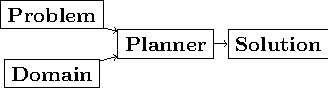
\includegraphics[width=.9\linewidth]{../img/pddl-workflow.pdf}
\caption{\label{fig:workflow}PDDL Planning workflow}
\end{figure}

A planner and use the generated solution file (\emph{plan}).

PDDL was first described in PDDL-the planning domain definition
language (1998) and has been in constant development since then.
This thesis makes use of \textcite{pddl3.1} if not otherwise stated. 

PDDL planning task specifications are composed of two separate text files:

\begin{itemize}
\item Domain file: description of general types, predicates, functions
and actions -> uninstanciated problem independent
\item Problem file: description of a concrete problem environment -> instance specific
\end{itemize}

This separation allows for an intuitive process of task modeling:
While general instances are described in the domain file, a specific
instance of a problem is created in the problem file.

These two files shell be investigated further in the following
sections.
\section{Format of the Domain File}
\label{sec-5-3}
The description of the task files is deliberately performed without
the use of the BNF notation. Fox et al. describe the BNF notation for
PDDL 2.1 in \cite{fox2003pddl2} as well as in Kovacs' (unpublished)
paper \cite{kovacs2011bnf}.


Domain files have a strict format: All keyword arguments must appear
in the order specified in the manual (an argument may be omitted) and
just one PDDL definition (of a domain, problem, etc.) may appear per
file. \cite[6]{fox2003pddl2}.

\subsection{{\bfseries\sffamily TODO} Include simple domain -> \LaTeX{}}
\label{sec-5-3-1}
\subsection{{\bfseries\sffamily TODO} Include simple problem -> \LaTeX{}}
\label{sec-5-3-2}
\subsection{{\bfseries\sffamily TODO} Include simple plan -> not yet in \LaTeX{}}
\label{sec-5-3-3}
\subsection{Define}
\label{sec-5-3-4}
Every domain file start with (define (domain <domainName>) \ldots{}) where,
<domainName> can be any string
\subsection{Requirements}
\label{sec-5-3-5}
The requirements part is not a mandatory part of a PDDL domain file.
However, as most planners only support a subset of PDDL they are
useful for determining if a planner is able to act on a given problem.
They are declared by the (:requirements \ldots{}) part. Some often used
requirements include \ldots{}
\subsection{Types}
\label{sec-5-3-6}
In order to assign to assign categories of objects, PDDL allows for
type definition. Like that, parameters in actions can be typed, as
well as arguments in predicates, functions [extra source!]. Later, in
the problem file, objects will be assigned to types, like objects to
classes in Object Orientated Programming (OOP). Adding to the (:requirement \ldots{}) part of
the file guarantees, that typing can be correctly used.
Strips (no types) vs ADL (types).
\subsection{Functions}
\label{sec-5-3-7}
Functions are not supported by many planners (source!) and, before
PDDL 3.1 they could only be modeled as 

\begin{center}
\fbox{
\begin{minipage}[c]{.6\textwidth}
Complete that!

\rule[.8em]{\textwidth}{2pt}

nil\end{minipage}
}
\end{center}


It is notable that before PDDL 3.0 the keyword functors was used instead
\subsection{Actions}
\label{sec-5-3-8}
PDDL 3.1 supports two types of actions: durative-action and the
'regular' action.
\section{Format of the Problem File}
\label{sec-5-4}
\section{Format of the Solution File (Plan)}
\label{sec-5-5}
\section{Planning Process}
\label{sec-5-6}
\chapter{Possibilities and Limitations}
\label{sec-6}
\section{Kitchen Domain}
\label{sec-6-1}
In this section, a kitchen domain will be presented, whereby PDDL
structures are presented that will be also useful in other domains. I
will start with a rather simple domain, present possible limitations
and then extend the file by more sophisticated constructs.
\subsection{Functions}
\label{sec-6-1-1}
As functions have a return value, the modeling possibilities
dramatically increase.

\subsection{Numerical Expressiveness}
\label{sec-6-1-2}
One might assume that the distance could be modeled as follows:

\begin{verbatim}
(durative action ...
...
  :duration (= ?duration (sqrt (coord-x )))
...
\end{verbatim}

However, PDDL does only support basic arithmetic operations (+, -, /, *).

An Euclidean distance function that uses the square root would be
convenient for distance modeling and measurement. However, PDDL 3.1
supports only four arithmetic operators (+, -, /, *). These
operators can be used in preconditions, effects
(normal/continuous/conditional) and durations.
\textcite{parkinson2012increasing} describe a workaround for this
drawback. By declaring an action `calculate-sqrt', they bypass the
lack of this function and rather write their own action that makes use
of the Babylonian root method.

\begin{enumerate}
\item Alternative \#1: Only sqrt exists
\label{sec-6-1-2-1}
Assuming that a function sqrt would actually exist, the duration could be modeled as follows:

\begin{verbatim}
:duration (= ?duration 
             (sqrt
              (+
               (*
                (- (pos-x (current-pos))
                   (pos-x ?goal))
                (- (pos-x (current-pos))
                   (pos-x ?goal)))
               (*
                (- (pos-y (current-pos))
                   (pos-y ?goal))
                (- (pos-y (current-pos))
                   (pos-y ?goal))))))
\end{verbatim}
\item Alternative \#2: sqrt and expt exist
\label{sec-6-1-2-2}
Assuming that a function sqrt would actually exist, the duration could be modeled as follows:
\begin{verbatim}
:duration (= ?duration 
             (sqrt
              (+
               (expt
                (- 
                 (pos-x (current-pos))
                 (pos-x ?goal)))
               (expt
                (- 
                 (pos-y (current-pos))
                 (pos-y ?goal))))))
\end{verbatim}

\item Alternative \#3: Calculate distance and hard code it, e.g. (distance table kitchen) = 5.9
\label{sec-6-1-2-3}

\begin{itemize}
\item Distance Matrix
\item \url{http://stackoverflow.com/questions/20654918/python-how-to-speed-up-calculation-of-distances-between-cities}
\item Scipy.spatial.distance (-> Clojure?)
\item Mention that the Taxicab geometry allows different ways that have an equal length
\end{itemize}

Another alternative is to make use of an external helper and, instead
of calculating every entry of the distance matrix. the distance only
if needed, incorporate every possible combination of two locations.
This approach has certainly a major drawback: With an increasing
amount of locations, the number of combinations increases
exponentially. That means, if there are 100 locations, there will be
\begin{center}
\fbox{
\begin{minipage}[c]{.6\textwidth}
TODO: Calculate possibilities

\rule[.8em]{\textwidth}{2pt}

nil\end{minipage}
}
\end{center}
\ldots{} . The native approach would be to iterate over the cities twice
and calculate only the half of the matrix (as it is symmetric, that
mean distance from A to B is the same as the distance from B to A).

\item Alternative \#4: Use the manhattan distance
\label{sec-6-1-2-4}

Allowing the agent to move only vertically and horizontally would be
that one can use the so called Taxicab geometry (or Manhattan length)
as distance measurement.  In the Kitchen domain, this could be modeled
as follows:

\begin{verbatim}
% => Metric: reduce duration

% dKitchenware.pddl 
\begin{figure}[t]
\inputminted[mathescape, linenos, numbersep=5pt, frame=lines, framesep=2mm]
            {csharp}
            {Code/dKitchenware.pddl}
\caption{The basic kitchenware domain}
\end{figure}
\section
\end{verbatim}
\item {\bfseries\sffamily TODO} Human Planner Interaction
\label{sec-6-1-2-5}


\item {\bfseries\sffamily TODO} World State - Plan Stepper
\label{sec-6-1-2-6}

\begin{itemize}
\item EMail + SMS connection
\item Very interesting: \url{http://www.tzi.de/~edelkamp/modplan/}
\end{itemize}

\item {\bfseries\sffamily TODO} Plan verification
\label{sec-6-1-2-7}
\% Reuse existing plans (VAL!). If a plan is not reusable, find
problems  (e.g. step 13 and 17) and try to find solutions for that
\item {\bfseries\sffamily TODO} Summary
\label{sec-6-1-2-8}
List all limits and possibilities and write 5 sentences for each
statement (my idea -> ask Alexandra).
\end{enumerate}
\chapter{Software Engineering Tools for AI Planning}
\label{sec-7}
\section{{\bfseries\sffamily TODO} Ideas}
\label{sec-7-1}
\begin{itemize}
\item PDDL type hierarchy and object instantiation to UML / TikZ, store
predicates (and action?) in same box as type
\item Research Knowledge Engineering in Planning
\item Human Computer Interaction
\begin{itemize}
\item \url{http://hci.waznelle.com/checklist.php}
\end{itemize}
\item Write Tiago (itSimple) regarding PDDL -> UML (and knowledge
engineering in general
\item ICKEPS (International Competition on Knowledge Engineering for
Planning and Scheduling)
\item Orient on "How to Design Classes"
\end{itemize}
\section{Statement of Problem}
\label{sec-7-2}
Writing and maintaining PDDL files can be time-consuming and
cumbersome \textcite{li2012translating}. So, the following development
tools shell support and facilitate the PDDL task design process and
reduce potential errors.

Below, methods are presented for

\begin{description}
\item[{Syntax Highlighting and Code Snippets}] Environment for Editing
PDDL files
\item[{Class Diagram Generator}] The automation of the PDDL task design process. File
input and output and dynamic generation (design level)
\item[{Human Planner Interaction}] An interactive PDDL environment: speech synthesis and
recognition.
\item[{Domain Generator}] Mathematical limitations (design level)
\end{description}
\section{Syntax Highlighting and Code Snippets}
\label{sec-7-3}


Writing extensive domain and problem files is a cumbersome task:
longer files can get quickly confusing. Therefore, it is convenient to
have a tool that supports editing these files. Syntax highlighting
describes the feature of text editors of displaying code in different
colors and fonts according to the category of terms (source: Wiki). A
syntax highlighting plug-in for the text and source code editors
\textcite{sublimetext2} and \textcite{sublimetext3} is proposed and
transferred to the on-line text editor Ace are used to implement this
feature, as ST Syntax Highlighting files can easily be converted to
Ace Files. 

For Mac user, TextMate (TM) is very similar to ST and the syntax
highlighting file can be used there, too. Besides, the general
principles (e.g. regular expressions) outlined here, apply to most of
other editors as well.  

\subsection{Implementation}
\label{sec-7-3-1}
ST syntax definitions are written in property lists in the XML format. 

The syntax definition is implemented by the use of the ST plug-in \textcite{aaapackagedev}. So, the definitions can be
written in YAML in converted to Plist XML later on. AAAPackageDEV provides the
following features:

\begin{quote}
AAAPackageDev is a Sublime Text 2 and 3 plug-in
that helps to create and edit syntax definitions, snippets,
completions files, build systems and other Sublime Text extensions.
\end{quote}

By means of Oniguruma regular expressions \parencite{kosako}, scopes are
defined, that determine the meaning of the PDDL code block. The scope naming
conventions mentioned in the \citetitle{textmate} are applied here. By the means
of the name, the colors are assigned. Different ST themes
display different colors (not all themes support all naming conventions).

The syntax highlighting is intended for PDDL 3.1, but is downward
compatible, as previous versions are subsets of later versions.
\begin{center}
\fbox{
\begin{minipage}[c]{.6\textwidth}
\textbf{\textsf{\textsc{TODO}}} Are later versions really subsets?

\rule[.8em]{\textwidth}{2pt}

nil\end{minipage}
}
\end{center}
Like that, the PDDL file is parsed 
\begin{center}
\fbox{
\begin{minipage}[c]{.6\textwidth}
\textbf{\textsf{\textsc{TODO}}} Is it really parsed, or are just parts highlighted?

\rule[.8em]{\textwidth}{2pt}

nil\end{minipage}
}
\end{center}
into different parts. 
\subsection{Usage and Customization}
\label{sec-7-3-2}
By using ST as editor, language independent ST features are supported, like auto
completion, code folding and column selection, described in the
Sublime Text 2 Documentation.

To enable syntax highlighting and code snippets, the files of the
repository have to be placed in the ST packages folder. The first part
of the PDDL.YAML-tmlanguage describes the parts of the PDDL task that
should be highlighted. By removing (or commenting) include statements,
the syntax highlighter is adjustable the user's need.

By default, all scopes are included.

\begin{enumerate}
\item Related Work
\label{sec-7-3-2-1}
\begin{enumerate}
\item PDDL Studio
\label{sec-7-3-2-1-1}
PDDL Studio \parencite{plch2012inspect} is an Integrated Development Environment (IDE) for
creating PDDL tasks. 

\item PDDL Mode
\label{sec-7-3-2-1-2}
Announced 2005 in a mailing list entry, PDDL mode supports PDDL 2.2. 
\item itSIMPLE
\label{sec-7-3-2-1-3}

\item Pygments
\label{sec-7-3-2-1-4}
\end{enumerate}
\end{enumerate}

\subsection{Evaluation}
\label{sec-7-3-3}
\section{Class Diagram Generator}
\label{sec-7-4}

The code is written in Clojure, a LISP dialect. As PDDL has a
'LISP-like syntax', using a LISP dialect for the interface is
convenient. This thesis uses Clojure[TODO: src], a relatively modern
LISP dialect that runs on the Java Virtual Machine. 

In order to start the document, a namespace has to be defined. The
required packages are:
\begin{description}
\item[{clojure.tools.reader.edn}] Safe file input. I will use this
method for entirely replacing the tools in clojure.core/read
\item[{clojure.java.io}] Methods for file input and output (IO)
\end{description}

\begin{verbatim}
(ns org-ba.core
  (:gen-class)
  (require [clojure.tools.reader.edn :as edn]
           [clojure.java.io :as io]
           [clojure.pprint :as pprint]
           [speech-synthesis.say :as say]
           [speech-recognition.hear :as hear]))
\end{verbatim}

\begin{verbatim}
#'user/a
\end{verbatim}

As PDDL files and 'information' will be in stored externally, a reader
method is needed. Edn reader provides functionality and guarantees
that no harmful commands can be read in through the reader
interface.

\begin{verbatim}
(defn read-lispstyle-edn
  "Read one s-expression from a file"
  [filename]
  (with-open [rdr (java.io.PushbackReader. (clojure.java.io/reader filename))]
    (edn/read rdr)))
\end{verbatim}

Next, a macro is provided for writing to files. It rebinds \textbf{out} to a
writer (that open a file for writing). Therefore, print statements
(print, prn, etc.) that normally would be send to the standard out,
are redirected to the file.

\begin{verbatim}
(defmacro write->file
  "Writes body to the given file name"
  [filename & body]
  `(with-open [w# (writer ~filename)]
     (binding [*out* w#]
       ~@body))
  (println "Written to file: " ~filename))
\end{verbatim}

Desired objects that belong to a type for a domain are sometimes
provided in a plain list, like the following:

\begin{verbatim}
vw-passat
opel-corsa
chevrolet-volt
\end{verbatim}

It would be convenient to add a type to these objects, for two
reasons:
\begin{itemize}
\item Add a super-type to the subtypes in the list
\item Add a type to a list of objects for the problem file
\end{itemize}

The following method affords that:
\begin{verbatim}
(defn read-objs
  "Read PDDL objects from a file and add type
  (e.g. 'table bed' -> (list table - furniture
                        bed - furniture))"
  [file object-type]
  (as-> (slurp file) objs
        (clojure.string/split objs #"\s")
        (map #(str % " - " object-type) objs)))
\end{verbatim}

By the help of these methods, you can create PDDL templates, for
example for a domain file:

\begin{verbatim}
(defn create-pddl
  "Creates a PDDL file from a list of objects and locations"
  [objs-file objs-type]
  (str
"(define (domain domainName)

  (:requirements
     :durative-actions
     :equality
     :negative-preconditions
     :numeric-fluents
     :object-fluents
     :typing)

  (:types\n"
   (pprint/cl-format nil "~{~&~5@T~a~}" (read-objs objs-file objs-type))
        ")

  (:constants

  )

  (:predicates

  )

  (:functions

  )

  (:durative-action actionName
     :parameters (?x - <objectType>)
     :duration (= ?duration #duration)
     :condition (at start <effects>)
     :effect (at end <effects>))
)"
))
\end{verbatim}

PDDL widely supports 'types'. These define possible shapes for objects
(similar to 'classes' in object oriented programming (OOP)). Types are
defined in the ':types' section of the PDDL domain file:
\begin{verbatim}
....
(:types man woman - human
        human - agent
        robot - agent)
...
\end{verbatim}

A meaning-full type hierarchy is the basis for clean, well-written
domains. Type definitions constitute the first part in the PDDL
domain design process, as they determine, on which possible objects
actions can be performed. 

In order to further work with the specified types, they have to be
extracted from the PDDL file. For this task, a regular expression is
used, that splits the types in subtypes and belonging types.

\begin{verbatim}
(defn split-up
  "Split a PDDL type list (:types obj1.1 obj1.2 - objT1 obj2 - objT2 ...)
  into strings of subtypes and associated types,
  [[subytype1 subtype 2 ... - type][subtype1 subtype2 ...][type]"
  [coll]
  (let [coll (if (= :types (first coll))
                 (rest coll)
                 coll)]
    ;; REVIEW: insert (\w) for trimming?
  (re-seq #"((?:\s*\w+\s*)+)-\s*(\w+)\s*"
        (clojure.string/join " " coll))))
\end{verbatim}

The resulting list can be used for creating a hash-map, where every
type from the PDDL type declaration is the hash-key and the subtypes
are the values. 

\begin{verbatim}
(defn types->hash-map
  "Convert splitted type list (['<expr>' '<subtype1.1> <subtype1.2> ...' '<type1>']
  to a hash-map {'<type1>': ['<subtype1.1>' '<subtype1.2>' ...], '<type2>': ...}"
  [coll]
  (reduce (fn [h-map [_ objs obj-type]]
           (let [key-obj-type (keyword obj-type)
                 existing-vals (key-obj-type h-map)]
          (assoc h-map
                 key-obj-type
                 (concat existing-vals
                       (clojure.string/split objs #"\s")))))
          {}
          coll))
\end{verbatim}

Now, as these information is present in a 'native' Clojure data
structure, it can be used for various purposes. A desirable purpose
would be to display the type hierarchy in kind of a 'class' diagram:

\begin{verbatim}
(defn map-entry->TikZ-seq
  "Converts a hashmap entry (:key [val1 val2 ...])
to a TikZ string (key -- { val1, val2 })"
  [entry]
(str
 (name (key entry))
        " -- "
        "{" (clojure.string/join ", " (val entry)) "}"))
\end{verbatim}

\begin{verbatim}
#'user/map-entry->TikZ-seq
\end{verbatim}

This method can now be used in order to create a TikZ standalone \LaTeX{}
file, that is converted to a png file by the use of lualatex.

\begin{verbatim}
(defn hash-map->TikZ-out
  "Converts complete PDDL type hash-map to TikZ file"
  [h-map]
  (str
"\\documentclass[tikz]{standalone}

\\usepackage[utf8]{inputenc}

\\usepackage{tikz}

\\usetikzlibrary{graphdrawing}
\\usetikzlibrary{graphs}
\\usegdlibrary{layered,trees}

\\begin{document}

\\begin{tikzpicture}

\\graph[layered layout, nodes={draw,circle,fill=blue!20,font=\\bfseries}]
{
  " (clojure.string/join ",\n  " (map map-entry->TikZ-seq h-map))
"
};

\\end{tikzpicture}
\\end{document}"))
\end{verbatim}

A resulting example image would look like this:

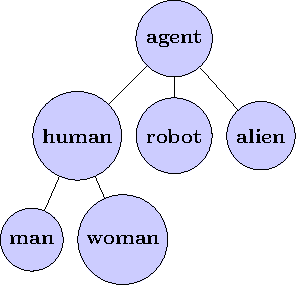
\includegraphics[width=.9\linewidth]{../img/tikz-file.pdf}

This look can be further extended in order to create a 
UML class diagram for PDDL domains and problems:

At last, a main method is used, that allows for testing and running the
script. 

\begin{verbatim}
(defn -main
  "Runs the input/output scripts"
  [& args]
  (print
   (types->hash-map
    (split-up
     '(:types man woman - agent table bed - furniture robot agent))))
  (say/say "Welcome to PDDL environment"))
\end{verbatim}

\section{VAL Plan Verification}
\label{sec-7-5}

\chapter{Evaluation}
\label{sec-8}
\chapter{Discussion}
\label{sec-9}
\chapter{Conclusion}
\label{sec-10}
\begin{verbatim}
(define (domain xyz)
  (:requirements
   :strips))
\end{verbatim}

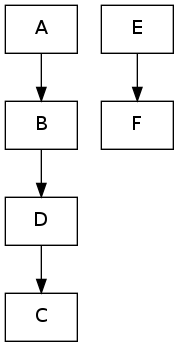
\includegraphics[width=.9\linewidth]{mygraph.png}
\chapter{Bibliography}
\label{sec-11}
\printbibliography

\chapter{Appendix}
\label{sec-12}
\(\alpha\)
% Emacs 24.3.1 (Org mode 8.2.5h)
\end{document}
